\documentclass[11pt]{article}

\usepackage[margin=1in]{geometry}
\usepackage{graphicx}
\usepackage{booktabs}
\usepackage{float}
\usepackage{hyperref}

\hypersetup{colorlinks=true, urlcolor=blue, linkcolor=black}

\title{AI651 / CS434 / EE5108\\ Assignment 1}
\author{Roll number 25280016\\ Name: \underline{\hspace{2.2in}}}
\date{5 October 2026}

\begin{document}
\maketitle

\noindent\textbf{GitHub repository (must be public):} \underline{\hspace{3.4in}}

\vspace{0.4em}
\noindent Task 1 numbers below are copied from the executed full-preset notebook (CUDA, 6{,}000 training steps). Task 2 numbers are copied from the validation table and the submission notes. The plots are the notebook outputs those answers discuss.

\section*{Response 1A}
\textbf{Question.} Before Output 1.1, record the expected order of the four forecasters for stations 1--3 and for held-out station 4. Then compare both station groups and Products A, B, and C, quantify the gaps, revise the order if needed, and explain the gaps from each model's assumptions.

\textbf{Answer.} Before the run, the expected order from best to worst was Period-routed ridge, then Raw Attention, then the two plain ridge models. Sensor-specific ridge cannot run on station 4, because that station was never used for fitting.

The measurements keep that order. Validation error is in m/s\(^{2}\).

\begin{table}[H]
\centering
\small
\begin{tabular}{lrrrr}
\toprule
Model & Stations 1--3 RMSE & Station 4 RMSE & Parameters & Fit time (s) \\
\midrule
Period-routed ridge & 0.166 & 0.173 & 59{,}904 & 0.034 \\
Raw Attention & 0.438 & 0.637 & 368{,}368 & 75.092 \\
Shared ridge & 0.767 & 0.876 & 4{,}608 & 0.030 \\
Sensor-specific ridge & 0.768 & unavailable & 13{,}824 & 0.109 \\
\bottomrule
\end{tabular}
\caption{Output 1.1. Validation RMSE. Lower is better.}
\end{table}

Period-routed ridge is also best on every product. On stations 1--3 its Product A / B / C errors are 0.181 / 0.164 / 0.152. Raw Attention is 0.422 / 0.474 / 0.415. Shared ridge is 0.805 / 0.854 / 0.621. On station 4, Period-routed ridge stays at 0.184 / 0.182 / 0.150, while Raw Attention stays at 0.646 / 0.599 / 0.663.

On stations 1--3, Raw Attention's error is about 2.6 times the period-routed error. Shared ridge is about 4.6 times worse. A separate matrix for each station changes almost nothing: 0.768 against 0.767.

Shared ridge uses one fixed map for every window, so a fast Product A cycle and a slow Product C cycle have to share one rule. Sensor-specific ridge only splits that map by station. The same station still changes pace every 192 samples, and station 4 has no map. Period-routed ridge estimates the pace of the current window and picks a map trained on that pace. Raw Attention can build a new mix for each window. It beats the two plain ridge models, and it does not catch the model that is given the pace directly.

\section*{Response 1B}
\textbf{Question.} Use Output 1.2 to show why one fixed map must compromise when the same station runs at two paces, and point to the phase or shape. Use Output 1.3 to show how the same learned projections can still produce different attention weights. Do not claim that attention recovered the physical period.

\textbf{Answer.} Output 1.2 is station 1 under two runs. Product A has period 16.135 samples. Product C has period 30.093 samples. Shared ridge has window RMSE 0.779 on the fast run and 0.448 on the slow run. On Product A its forecast is too smooth, and its peaks do not line up with the truth. On Product C the slower wave is closer to a middle shape, so the same map looks better, but the peaks are still flattened. Period-routed ridge follows both runs, with window errors 0.232 and 0.150. One matrix cannot advance the phase by both 16 and 30 samples.

\begin{figure}[H]
\centering
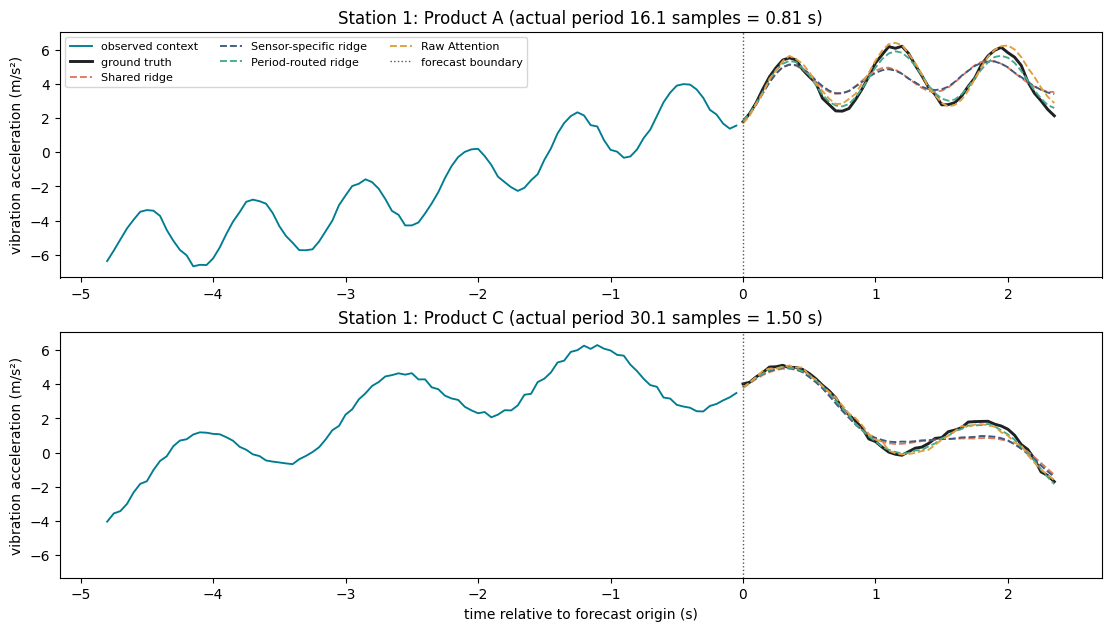
\includegraphics[width=\textwidth]{figures/output-1-2.png}
\caption{Figure 1. Output 1.2. Station 1 under Product A and Product C.}
\end{figure}

Output 1.3 uses the same learned projections on those two windows. The attention maps differ. The mean absolute weight difference is 0.012, and the largest difference is 0.454. The same projections therefore build a different mix when the window changes. The figure does not show that attention found the 16-sample or 30-sample period.

\begin{figure}[H]
\centering
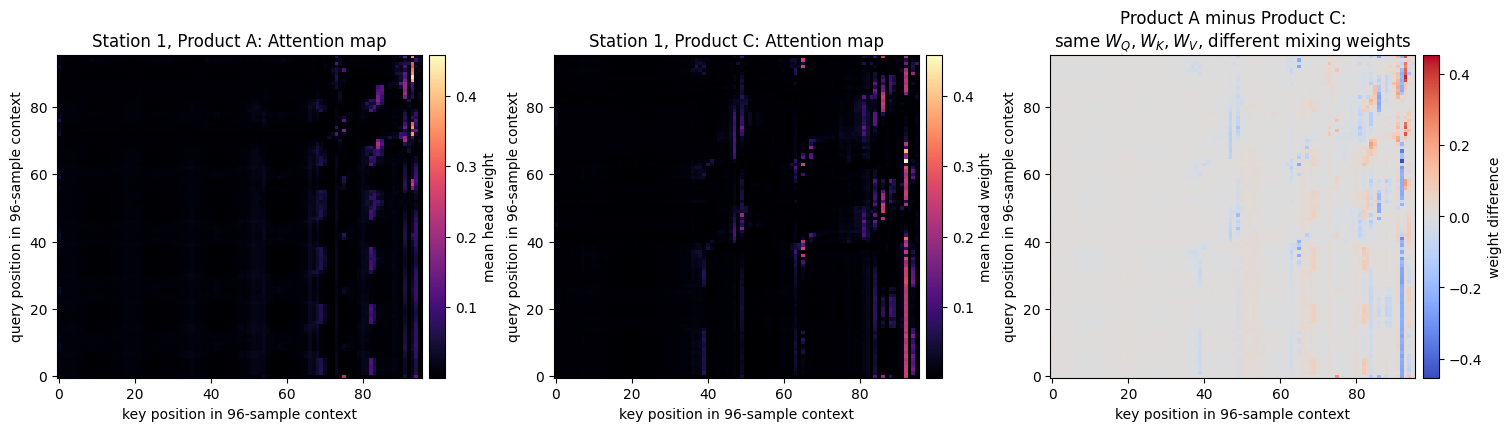
\includegraphics[width=\textwidth]{figures/output-1-3.png}
\caption{Figure 2. Output 1.3. Attention weights for the same station under two products.}
\end{figure}

\section*{Response 2}
\textbf{Question.} State the selected moving-average width. Describe what changes in Outputs 2.1--2.3, including the validation comparison of Raw Attention and Attention plus decomposition. Explain why a moving average fits this drift-plus-vibration signal, and why the training-only period check is a fair way to choose the width. Give one case where this bias fails, or name another decomposition and the assumption it would make.

\textbf{Answer.} The selected width is 41 samples.

In Output 2.1, a narrow average follows the wiggles, so they fall into the trend and the leftover is small. At width 17 the leftover has standard deviation 0.578. At width 41 the trend is the slow ramp, and the leftover keeps a clean wave with standard deviation 1.572. On the plotted Product C window, whose true period is 32 samples, the width-41 leftover has a sharp period score at that period. The raw window's period score is almost flat.

\begin{figure}[H]
\centering
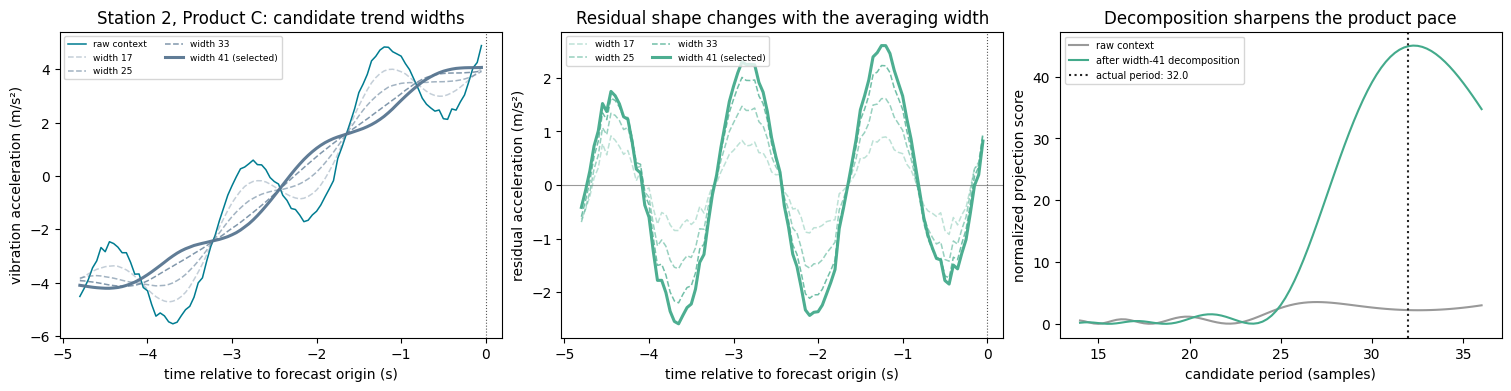
\includegraphics[width=\textwidth]{figures/output-2-1.png}
\caption{Figure 3. Output 2.1. Trend and leftover at candidate widths. Width 41 is selected.}
\end{figure}

Output 2.2 scores how often the leftover's period is within one sample of the true period. This check only chooses the width. The true period is not given to the forecaster. Recovery rises from 0.687 on the raw window to 0.980, 0.989, 0.993, and 0.998 at widths 17, 25, 33, and 41. Width 41 is best on that score, so it is the width used. Its median absolute period error is 0.216 samples, which is a little larger than width 25 (0.122). The selection rule was recovery within one sample, not the median error.

Output 2.3 shows that the split helps every product. Validation RMSE on stations 1--3 falls from 0.438 for Raw Attention to 0.304 for Attention plus decomposition. On station 4 it falls from 0.637 to 0.457. By product, stations 1--3 go from 0.422 / 0.474 / 0.415 to 0.284 / 0.337 / 0.287.

A moving average fits because the slow drift changes over about 240 samples. Inside a 96-sample window it looks like a smooth ramp, while the vibration repeats every 14--36 samples. An average of width 41 follows the ramp and leaves the vibration behind. The encoder then sees the vibration, and a linear head forecasts the ramp.

This bias would fail on a sudden jump in level. The average would smear that jump across 41 samples and treat part of it as vibration. A Hodrick--Prescott smoother would instead assume the trend bends smoothly. It can keep a jump sharper, and it gives up the simple moving average and the exact leftover-plus-trend split.

\section*{Response 3}
\textbf{Question.} Confirm the delay-score check and the aggregation example. From Output 3.2, which lags repeat most strongly, and how do they relate to the run's period? Why is the leftover cleaner than the raw signal, and why does that support delay mixing? Describe one signal for which a few repeating delays would be the wrong bias. Do not call the figure a plot of the trained model's scores.

\textbf{Answer.} Output 3.1 checks the series \([1, 3, 1, 3]\). The FFT delay scores are \([4, -4, 4, -4]\), the same as the direct circular correlation. The aggregation example uses values \([10, 20, 30, 40]\), delays 1 and 3, and weights 0.75 and 0.25. The mixed result is \([35, 15, 25, 25]\). The first value is 35, so each delay reads backward: position \(t\) uses the value from \(t\) minus the delay.

Output 3.2 is station 2 during a Product A run whose true period is 16.135 samples. The strongest leftover correlations are 0.896 at delay 16 and 0.897 at delay 32. Those are one period and two periods. The raw-signal correlation does not have those peaks. It is one broad hump, because a rising drift still looks like itself after many shifts.

Removing the drift makes peaks line up with peaks at the real spacing. That is the reason to decompose first and then mix by delay. The figure is a correlation of the signal itself. It is not the model's learned delay scores.

Delay mixing is the wrong bias for a one-off spike, or for a pace that changes inside one 96-sample window. It copies the same few shifts across the whole window. A spike would be pasted again one period later, and a changing pace would be forced onto one spacing.

\begin{figure}[H]
\centering
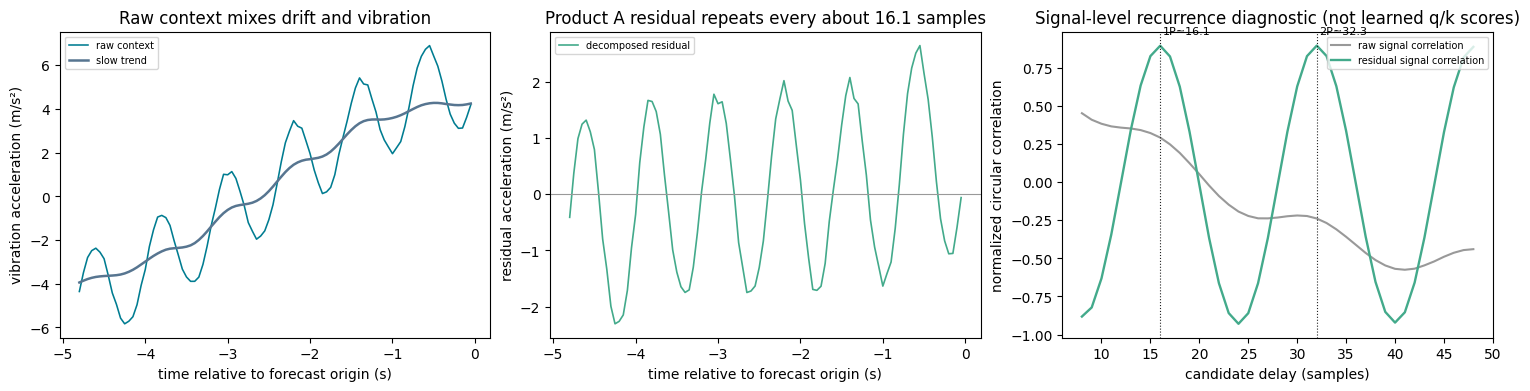
\includegraphics[width=\textwidth]{figures/output-3-2.png}
\caption{Figure 4. Output 3.2. Signal-level recurrence, not learned query/key scores.}
\end{figure}

\section*{Response 4}
\textbf{Question.} (a) In at most two sentences, before Output 4.1, say which upgrade should help most when the slow part is large, and why. (b) Report the validation RMSEs and MSEs, compare the two architectural switches, and summarize how error changes across the 48-step horizon. (c) Choose the deployment model for stations 1--3 and for station 4 using validation error, parameter count, and fit time.

\textbf{Answer.}

\begin{table}[H]
\centering
\small
\begin{tabular}{lrrrr}
\toprule
Model & St.\ 1--3 RMSE & St.\ 1--3 MSE & St.\ 4 RMSE & St.\ 4 MSE \\
\midrule
Period-routed ridge & 0.166 & 0.028 & 0.173 & 0.030 \\
Autoformer-inspired & 0.198 & 0.039 & 0.242 & 0.059 \\
Raw delay mixer & 0.224 & 0.050 & 0.331 & 0.109 \\
Attention + decomposition & 0.304 & 0.092 & 0.457 & 0.209 \\
Raw Attention & 0.438 & 0.192 & 0.637 & 0.405 \\
Shared ridge & 0.767 & 0.588 & 0.876 & 0.767 \\
Sensor-specific ridge & 0.768 & 0.590 & unavailable & unavailable \\
\bottomrule
\end{tabular}
\caption{Outputs 1.1 and 4.1. Validation error for every fitted model.}
\end{table}

% BEGIN RESPONSE 4 INTERPRETATION
\noindent Where the slow ramp is large, decomposition should help most, because it takes that ramp out of the mixer. Delay mixing helps the repeating part, but it does not remove the ramp.

\noindent On stations 1--3, delay mixing alone cuts Raw Attention's RMSE by 0.214. Decomposition alone cuts it by 0.134. Both together cut it by 0.240, which is less than \(0.214 + 0.134\). The two gains overlap, and delay mixing is the stronger single upgrade. Station 4 shows the same pattern. In Output 4.2, every model gets worse from step 1 to step 48, and the rise is steeper on station 4. Period-routed ridge stays lowest. Raw Attention rises the most.

\noindent Period-routed ridge is the deployment choice for both groups. It has the lowest validation error, 59{,}904 parameters, and a fit time of 0.034 seconds. Autoformer-inspired is the best neural model, but it is less accurate, uses 373{,}026 parameters, and takes 192 seconds. Sensor-specific ridge cannot be used on station 4. On the final test data, Period-routed ridge scores 0.161 on stations 1--3 and 0.183 on station 4.
% END RESPONSE 4 INTERPRETATION

\begin{figure}[H]
\centering
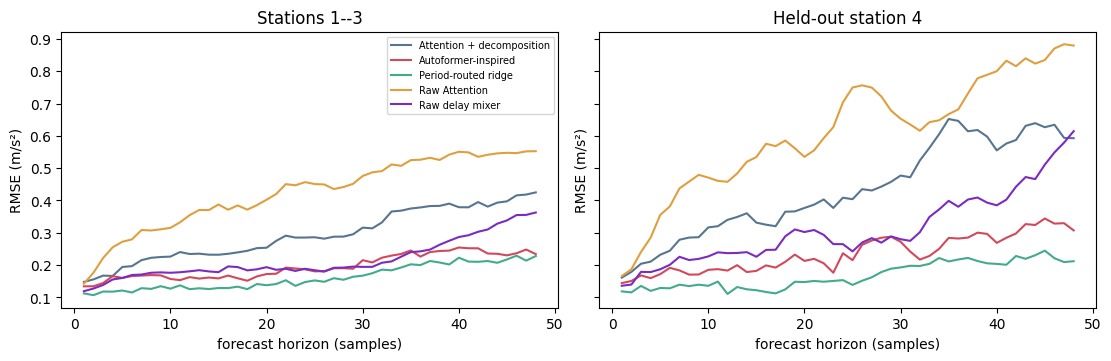
\includegraphics[width=\textwidth]{figures/output-4-2.png}
\caption{Figure 5. Output 4.2. RMSE at each step of the 48-step horizon.}
\end{figure}

\begin{figure}[H]
\centering
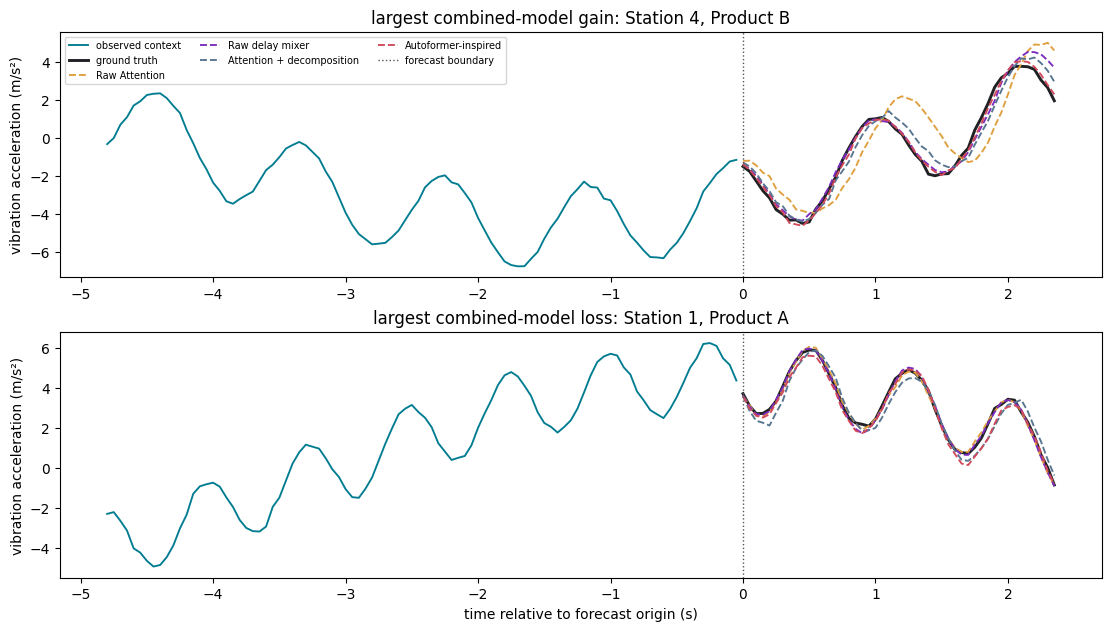
\includegraphics[width=\textwidth]{figures/output-4-1.png}
\caption{Figure 6. Output 4.1. The window where the combined model gains the most, and the window where it loses.}
\end{figure}

\section*{Task 2}
\textbf{What the report asks.} Describe the preprocessing, the model, and the reasons for those choices. Compare the optional external file on and off, on more than one seed, using a time-ordered validation split. State the parameter count and epoch count submitted to the leaderboard.

\textbf{Answer.} The history has 43{,}656 values. The forecast is the next 168 values, \texttt{time\_idx} 43657 through 43824. The target is never negative. Its mean is about 98, and its level can jump sharply inside one 168-step block. On the last four blocks of 168 steps, copying the last value has RMSE 245.2. Copying the last 24 steps has RMSE 175.5.

The past is placed on a log scale, using a mean and spread fit only on the history available at that stage. The six continuous external columns are scaled the same way. The four on/off columns are left as 0 or 1. External values over the 168 future steps are fed to the forecast. The handout allows this, because those values are not the target. A 14-day average of each hour of the day is also given to the model, so one unusually quiet final day does not set the whole week.

The submitted model is an Autoformer. A moving average of width 25 splits each window into a smooth part and a leftover. An FFT correlation finds the strongest delays, and the leftover is mixed from those shifted copies. That is delay mixing, not ordinary attention. A direct reading of the future external values and the hour-of-day shape makes the main guess. The network adds a correction. A softplus keeps every forecast at least zero. The context length is 336, the width is 32, and there are 2 layers. The training loss is raw squared error, because the leaderboard scores raw RMSE.

The check uses the last four non-overlapping blocks of 168 steps. Two seeds agree.

\begin{table}[H]
\centering
\small
\begin{tabular}{lrrrrrr}
\toprule
External file & Seed & RMSE & MAE & sMAPE & Best epoch & Parameters \\
\midrule
Off & 0 & 96.65 & 79.31 & 101.43 & 8 & 54{,}663 \\
Off & 1 & 96.65 & 79.57 & 101.73 & 3 & 54{,}663 \\
On & 0 & 69.39 & 49.54 & 78.61 & 10 & 55{,}280 \\
On & 1 & 69.67 & 49.70 & 79.84 & 9 & 55{,}280 \\
\bottomrule
\end{tabular}
\caption{Task 2 ablation on the chronological validation blocks.}
\end{table}

The external file lowers the check error by about 27 RMSE points for both seeds, so the submitted forecast uses it. The two seeds were refit and their 168-step forecasts were averaged. The leaderboard entry declares \textbf{110{,}560 parameters} and \textbf{20 epochs}. That is the submission at rank 38.

\section*{Generative AI disclosure}
A coding assistant in Cursor was used for this assignment. It was asked to implement the three notebook functions, to write the Task 2 Autoformer script, and then to draft these responses from the full-run notebook and the Task 2 output files. The Task 1 numbers were taken from that notebook. The Task 2 numbers were taken from the validation table and the submission notes. After the first leaderboard submission, the Task 2 script was changed so the forecast is trained on the raw error, is not glued to the last day, and starts from the external features and the hour-of-day shape. The responses above were edited to follow those measured outputs.

\end{document}
